
\chapter{Framework Automated Tuning \label{chap:05-Framework_parameter_tuning}}

% First paragraph has no indentation.

\noindent The models and algorithms from Chapter~\ref{chap:04-Framework-design-and-implementation}
constitute the basis for the radio-coverage framework used throughout
this thesis. Until here, the framework has been studied in the context
of optimization-problem solving for radio networks. In this chapter,
the focus is shifted towards radio-network planning activities, and
how the framework can aid a network-planning engineer in his or her
everyday tasks. The objective is to facilitate refined network planning,
the complexity of which is generally beyond the scope of any manual
approach.

A central part of a radio-planning tool is its radio-propagation model.
Generally speaking, the signal-propagation predictions will be as
good as the input data used for their estimation. Moreover, acquiring
and constantly upgrading the necessary data to support the decision
making in this context is an expensive and challenging task. In practical
situations, an emitted signal propagates by interacting with the surrounding
environments. Consequently, the ability of a propagation model to
adapt to the environment where it is used improves the accuracy of
the calculated signal-propagation predictions.

In this context, this chapter presents two automated-tuning capabilities
for PRATO. The first one involves the parameter tuning of the empirical
radio-propagation model using a snapshot of field measurements. The
second one involves the optimization of clutter losses over different
regions of the country, therefore adapting the loss factors to the
local conditions of each region. The results of the experimental simulations,
performed over three regions of the real LTE network deployed by Telekom
Slovenije, d.d., show the suitability of the presented methods to
improve the accuracy of the calculated radio-propagation predictions.

To the best of the author's knowledge, there is no reference in the
literature of an optimization-based approach to automatically adapt
the signal losses due to clutter. The content of this chapter extends
the research work published by the author in~\cite{Benedicic-An_adaptable_parallel_simulation_framework_for_LTE_coverage_planning:2013}. 

The rest of this chapter is organized as follows. Section~\ref{sec:05-Motivation}
describes the benefits of the presented approach from the radio-planning
point of view. After giving an overview of relevant publications in
Section~\ref{sec:05-Related_work}, the parameter-tuning problem
and the analytical approach for solving it are presented in Section~\ref{sec:05-Parameter_tuning_radio-propagation_model},
including the experimental simulations and their results. Section~\ref{sec:05-Clutter_optimization}
concentrates on the description of the optimization problem involving
the regional adaptation of signal losses due to clutter, including
an extensive analysis of the performed simulations on three test networks.


\section{Motivation \label{sec:05-Motivation}}

With the advent of LTE as part of the 4G in cellular technology, mobile
operators are facing the challenges of deploying a new network. LTE
follows the well established UMTS/HSPA combo, targeting higher peak
data rates, higher spectral efficiency and lower latency~\cite{Song_Evolved_cellular_network_planning_and_optimization_for_UMTS_and_LTE:2010}. 

The deployment of a new radio network is always a challenge for mobile
operators, who constantly struggle to find the optimal investment
in order to provide a competitive network in terms of coverage and
QoS. Indeed, coverage planning remains a key problem that all operators
have to deal with.

Although different mathematical models have been proposed for radio-propagation
modeling, none of them excels in a network-wide scenario~\cite{Shabbir_Comparison_of_radio_propagation_models:2011}.
Empirical propagation models usually give good results with a limited
computational effort. However, for improved accuracy, the model parameters
have to conform to a specific network or region within it, mainly
because of the inaccuracies in input data and the environmental changes
in the region, e.g., foliage of trees or snow. Consequently, a combination
of different parameters is generally needed in order to reliably calculate
radio-propagation predictions of large networks that cover different
environments.

To address the aforementioned issues, the parameters of an empirical
propagation model are adapted based on a set of field measurements.
The parameter tuning is analytically calculated per cell, in order
to increase the accuracy of the calculated predictions. Moreover,
by applying an optimization approach, the signal losses due to clutter
are automatically adjusted in a regional basis.

As a simulation framework to evaluate the presented problems, PRATO,
the parallel radio-prediction tool presented in Chapter~\ref{chap:04-Framework-design-and-implementation},
is used. Therefore, the suitability of the framework for network planning
and optimization of LTE radio networks is also validated. Specifically,
the tool should be capable of handling a large number of radio-propagation
predictions using a metaheuristic algorithm, and a distributed objective-function
evaluation.


\section{Related work \label{sec:05-Related_work}}

Following an optimization-oriented approach, the authors of \cite{Aarnaes-Tuning_of_empirical_radio_propagation_models_effect_of_location_accuracy:2004}
study the effects on location accuracy while performing semi-automated
optimization of the parameters of a radio-propagation model. While
their optimization component improves the accuracy of the radio predictions,
it does so requiring human intervention, hence the term semi-automated
optimization. In terms of the effects of location accuracy, they conclude
that locations with a median accuracy of around 60~m may be used
for parameter tuning. Also, they notice that although the model accuracy
improved after the parameter tuning, it gives inadequate results when
used for predicting radio propagation over distant areas.




\section{Parameter tuning of the radio-propagation model \label{sec:05-Parameter_tuning_radio-propagation_model}}

The effectiveness of the decision-making process during radio-network
planning is tightly coupled with the precision achieved by the propagation
model used. In order to obtain a radio-propagation model that most
accurately reflects the propagation characteristics of the area covered
by each radio cell in the network, the parameters of the mathematical
model are adapted to the target environment into which it is to be
used. Current state-of-the-art methods for such parameter tuning depend
on existing field-measurement data \cite{Aarnaes-Tuning_of_empirical_radio_propagation_models_effect_of_location_accuracy:2004,Yang_A_linear_least_square_method_of_propagation_model_tuning_for_3G_radion_network_planning:2008},
which are collected in advance for the area covered by the target
network. Starting from an a-priori best-known set of parameters, empirically
calculated by the radio engineers, this approach adapts the model
parameters so that the deviation of the radio-propagation prediction
to a given set of field measurements is minimized.

To calculate the radio-propagation predictions, the empirical model,
previously introduced in Section~\ref{sub:04-Radio_propagation_model},
is used. Recall that the model contains a vector of adaptable parameters,
$\vec{\beta}$. For this reason, this mathematical model is especially
appropriate for tuning, since it can be adapted to a given scenario
and its local conditions by adjusting the values of the vector $\vec{\beta}=(\beta_{0},\beta_{1},\beta_{2},\beta_{3})$,
the elements of which represent:
\begin{description}
\item [{$\beta_{0}$}] the reference loss or offset,
\item [{$\beta_{1}$}] the loss slope due to distance of the receiver from
the transmitter,
\item [{$\beta_{2}$}] the loss slope due to height of the transmitter
antenna, and
\item [{$\beta_{3}$}] the loss slope due to the combined effect of the
distance and height of the antenna.
\end{description}
The parameter tuning is performed per cell to improve the local fitting
of the radio predictions, being its resulting solution a vector $\vec{\beta}_{c}$
for a target cell $c$, $c\in C$.

Also, recall that the model includes an extra term in order to adequately
predict signal-loss effects due to foliage, buildings and other fabricated
structures. These loss factors are based on the land usage, known
as clutter data. Here, twelve different clutter categories are recognized.
Table~\ref{tab:05-Clutter_categories} lists these categories, including
their label numbers and descriptions. 

\begin{table}
\centering

\caption{Clutter-category label numbers and descriptions for the signal loss
due to clutter, as reflected by a radio-propagation model. \label{tab:05-Clutter_categories}}


\begin{tabular}{cl}
\hline 
Clutter category & Description\tabularnewline
\hline 
0 & Urban area without buildings, mostly roads\tabularnewline
1 & Suburban area \tabularnewline
2 & Urban area\tabularnewline
3 & Dense urban area\tabularnewline
4 & Agricultural area\tabularnewline
5 & Forestall area\tabularnewline
6 & Swamp area\tabularnewline
7 & Dry open land area with special vegetation\tabularnewline
8 & Dry open land area without special vegetation\tabularnewline
9 & Water area\tabularnewline
10 & Industrial area\tabularnewline
11  & Park area\tabularnewline
\hline 
\end{tabular}
\end{table}



\subsection{Field measurements \label{sub:05-Field_measurements}}

In radio networks, a UE constantly performs cell selection/reselection
procedures and handover (see Section~\ref{sub:02-Handover-and-soft-handover}),
in order to keep the best possible connection to the network. Within
this context, the best connection is selected by probing a QoS measure
of the neighboring cells. In LTE networks, the UE measures two parameters
from the reference signal of the network, namely the Reference Signal
Received Power (RSRP\nomenclature[A]{RSRP}{Reference signal received power})
and the Reference Signal Received Quality (RSRQ\nomenclature[A]{RSRQ}{Reference signal received quality}).

For a certain frequency bandwidth, RSRP measures the average received
power over the resource elements that carry cell-specific reference
signals. RSRP is applicable in both idle mode (e.g., waiting for a
call) and connected mode (e.g., during a call). During the procedure
of cell selection/reselection in idle mode, RSRP is used, whereas
RSRQ is only applicable when the UE is in connected mode. 

The radio-propagation prediction involves calculating the network
coverage over a certain region. Hence, in the first place, the focus
is on accurately predicting the best connection a UE would select
in idle mode and the RSRP measurements it uses.

Here, the field measurements representing the RSRP at a given location
were collected using a small truck that was equipped with a spectrum
analyzer. The spectrum analyzer was connected to an external omni
antenna mounted on the roof of the truck, at roughly 2~m above the
ground, taking measurements at a rate of 2~Hz. To accurately establish
the measurement-location points, a Global-Positioning-System (GPS\nomenclature[A]{GPS}{Global positioning system})
unit was used. These GPS-informed locations have been tested to be
compliant with the 60~m limit mentioned in~\cite{Aarnaes-Tuning_of_empirical_radio_propagation_models_effect_of_location_accuracy:2004}.
The measurements cover most of the streets within the target area,
with over 300,000 individual points, collected for more than 140 network
cells.

To minimize the error impact in measured RSRP, all field measurements
are processed so that a single value, the median, was calculated for
each of the measured locations. This processing step improves measured-data
quality in terms of possible deviations due to external factors, e.g.,
driving speed. The resulting RSRP was then used to estimate the path-loss
prediction at the corresponding location, the resolution of which
matches that of the DEM and clutter data used.


\subsection{Linear least squares \label{sub:05-Linear_least_squares}}

The approach for tailoring the radio-prediction model is to correlate
the field measurements with the predicted RSRP values. The new parameter
set originates from the minimization of an error criterion. Similar
to~\cite{Aarnaes-Tuning_of_empirical_radio_propagation_models_effect_of_location_accuracy:2004,Huang_Online_propagation_model_correction_based_on_PSO_algorithm_in_LTE_SON_system:2012,Yang_A_linear_least_square_method_of_propagation_model_tuning_for_3G_radion_network_planning:2008},
the minimization criterion is the squared-sum difference between the
predicted and the observed RSRP levels, i.e.:

\begin{equation}
E(\vec{\beta_{c}})=\sum_{i=1}^{m_{c}}(p_{c}-\mathrm{L}{}_{c}(i,\vec{\beta_{c}})-fm_{i})^{2},\label{eq:05-Least_squares_error}
\end{equation}


\noindent where $E(\vec{\beta_{c}})$ is the observed error (in dB)
for cell $c$ given the parameters $\vec{\beta_{c}}$, $p_{c}$ is
the pilot power of cell $c$, and $\mathrm{L}_{c}(i,\beta_{c})$ is
the path loss of cell $c$ at the same geographical point of $fm_{i}$,
i.e., the $i$-th field measurement out of a set of measurements for
cell $c$, the cardinality of which is $m_{c}$.

A necessary condition for the linear least-squares method to find
the global minimum is the linear relationship between the predicted
path loss, $\mathrm{L}{}_{c}(i,\vec{\beta})$, and the vector $\vec{\beta_{c}}$~\cite{Yang_A_linear_least_square_method_of_propagation_model_tuning_for_3G_radion_network_planning:2008}.
This condition can be verified by calculating the first derivative
of $E(\vec{\beta_{c}})$ in terms of the components of vector $\vec{\beta_{c}}=<\beta_{0c},\beta{}_{1c},\beta_{2c},\beta_{3c}>$,
i.e., $\frac{\partial E(\vec{\beta_{c}})}{\partial\beta{}_{0c}}=0$,
$\frac{\partial E(\vec{\beta_{c}})}{\partial\beta_{1c}}=0$, $\frac{\partial E(\vec{\beta_{c}})}{\partial\beta_{2c}}=0$,
and $\frac{\partial E(\vec{\beta_{c}})}{\partial\beta{}_{3c}}=0$.


\subsection{Simulations \label{sub:05-Simulations}}

The simulations consisted in building the matrices of the observed-error
values, $E(\vec{\beta_{c}})$, for each cell $c$ in the target network.
The linear systems of equations are then individually solved by applying
the linear least-squares method, which involves the evaluation of
one radio-coverage prediction per cell. Each solved system holds a
unique solution for a cell $c$, $c\in C$, denoted by the vector
$\vec{\beta_{c}}$.


\subsection{Test networks \label{sub:05-Test_networks}}

The test networks, Net$_{8}$, Net$_{9}$, and Net$_{10}$, are subsets
of a real LTE network deployed in Slovenia by Telekom Slovenije, d.d.
The path-loss predictions are calculated using PRATO, with a DEM and
clutter map of 25~m$^{2}$ resolution, and a receiver height of 2~m
above ground level. A transmission radius of 16~km defines the coverage
prediction area around each network transmitter, thus limiting the
path-loss prediction to a distance where it is feasible for a UE to
connect to a cell, with a RSRP greater or equal to -124~dBm~\cite{Neuland_Influence_of_Different_Factors_on_X_Map_Estimation_in_LTE:2011}.
At the same time, the selected transmission radius provides enough
overlap among neighboring cells to calculate the network coverage
over the whole region. Table~\ref{tab:05-Test_network_properties}
provides detailed information about the test networks used, showing
the number of network cells, the area surface, and the covering proportion
of the collected field measurements in terms of the total area of
each test network.

\begin{table}
\centering

\caption{Parameters of the test networks Net$_{8}$, Net$_{9}$ and Net$_{10}$
that were used for the experimental simulations during the automated
tuning of the radio-propagation model.\label{tab:05-Test_network_properties}}


\begin{tabular}{cccc}
\cline{2-4} 
 & Number of cells  & Area {[}km$^{2}${]} & Field-measurement proportion {[}\%{]}\tabularnewline
\hline 
Net$_{8}$  & 12 & 103.74 & 5.41\tabularnewline
Net$_{9}$  & 130  & 1298.02 & 12.02\tabularnewline
Net$_{10}$  & 6  & 386.38 & 2.30\tabularnewline
\hline 
\end{tabular}
\end{table}


Net$_{8}$ represents a network deployed over a dominant agricultural
area with almost flat terrain, some forests and water streams. Net$_{9}$
is deployed over a densely populated urban area, containing high buildings,
parks and avenues. The last one, Net$_{10}$, represents a network
deployed over hilly terrain, including some smaller villages and vast
forests. It is important to note that the number of deployed cells
is directly proportional to the population density within the region
of each test network (see Chapter~\ref{chap:02-Principles_of_mobile_radio_networks}).
This relationship can be derived from the information listed in Table~\ref{tab:05-Test_network_properties},
where the number of cells is shown along the area of every test network.
For a clearer characterization in terms of the terrain types and their
extent, the proportion of each clutter category with respect to the
total area of every test network is shown in Table~\ref{tab:05-Proportion_of_clutter_for_test_networks}.

\begin{table}
\centering

\caption{Clutter-category proportions, expressed in percent, in terms of the
surface area of each of the test networks. The category legend is
given in Table~\ref{tab:05-Clutter_categories}. \label{tab:05-Proportion_of_clutter_for_test_networks}}


{\scriptsize{}}%
\begin{tabular}{>{\centering}p{0.4cm}>{\centering}p{0.7cm}>{\centering}p{0.7cm}>{\centering}p{0.7cm}>{\centering}p{0.7cm}>{\centering}p{0.7cm}>{\centering}p{0.7cm}>{\centering}p{0.7cm}>{\centering}p{0.7cm}>{\centering}p{0.7cm}>{\centering}p{0.7cm}>{\centering}p{0.7cm}>{\centering}p{0.7cm}>{\centering}p{0.6cm}}
\cline{2-14} 
 & {\scriptsize{Cat.0}} & {\scriptsize{Cat.1}} & {\scriptsize{Cat.2}} & {\scriptsize{Cat.3}} & {\scriptsize{Cat.4}} & {\scriptsize{Cat.5}} & {\scriptsize{Cat.6}} & {\scriptsize{Cat.7}} & {\scriptsize{Cat.8}} & {\scriptsize{Cat.9}} & {\scriptsize{Cat.10}} & {\scriptsize{Cat.11}} & {\scriptsize{Total}}\tabularnewline
\hline 
{\scriptsize{Net$_{8}$ }} & {\scriptsize{0.53}} & {\scriptsize{4.53}} & {\scriptsize{1.68}} & {\scriptsize{0.45}} & {\scriptsize{71.89}} & {\scriptsize{17.94}} & {\scriptsize{0.07}} & {\scriptsize{0.00}} & {\scriptsize{0.03}} & {\scriptsize{2.21}} & {\scriptsize{0.67}} & {\scriptsize{0.00}} & {\scriptsize{100.00}}\tabularnewline
{\scriptsize{Net$_{9}$ }} & {\scriptsize{0.91}} & {\scriptsize{5.53}} & {\scriptsize{9.48}} & {\scriptsize{3.84}} & {\scriptsize{29.73}} & {\scriptsize{48.57}} & {\scriptsize{0.14}} & {\scriptsize{0.03}} & {\scriptsize{0.03}} & {\scriptsize{0.76}} & {\scriptsize{0.86}} & {\scriptsize{0.12}} & {\scriptsize{100.00}}\tabularnewline
{\scriptsize{Net$_{10}$ }} & {\scriptsize{0.15}} & {\scriptsize{3.99}} & {\scriptsize{1.14}} & {\scriptsize{0.11}} & {\scriptsize{26.50}} & {\scriptsize{67.13}} & {\scriptsize{0.26}} & {\scriptsize{0.00}} & {\scriptsize{0.00}} & {\scriptsize{0.36}} & {\scriptsize{0.36}} & {\scriptsize{0.00}} & {\scriptsize{100.00}}\tabularnewline
\hline 
\end{tabular}
\end{table}


Since the terrain profiles are most relevant for Net$_{8}$ and Net$_{10}$,
they are shown in Figures~\ref{fig:05-Terrain_profile_for_Net8}
and~\ref{fig:05-Terrain_profile_for_Net10}, respectively. Note that
the terrain shown in Figure~\ref{fig:05-Terrain_profile_for_Net8}
is mostly flat, since the agricultural area prevails in Net$_{8}$.
In contrast, the terrain for Net$_{10}$ is dominated by hills, which
are mostly covered by dense forests, including some small villages
in the valleys (see Figure~\ref{fig:05-Terrain_profile_for_Net10}).

\begin{figure}
\begin{minipage}[t]{0.49\textwidth}%
\centering

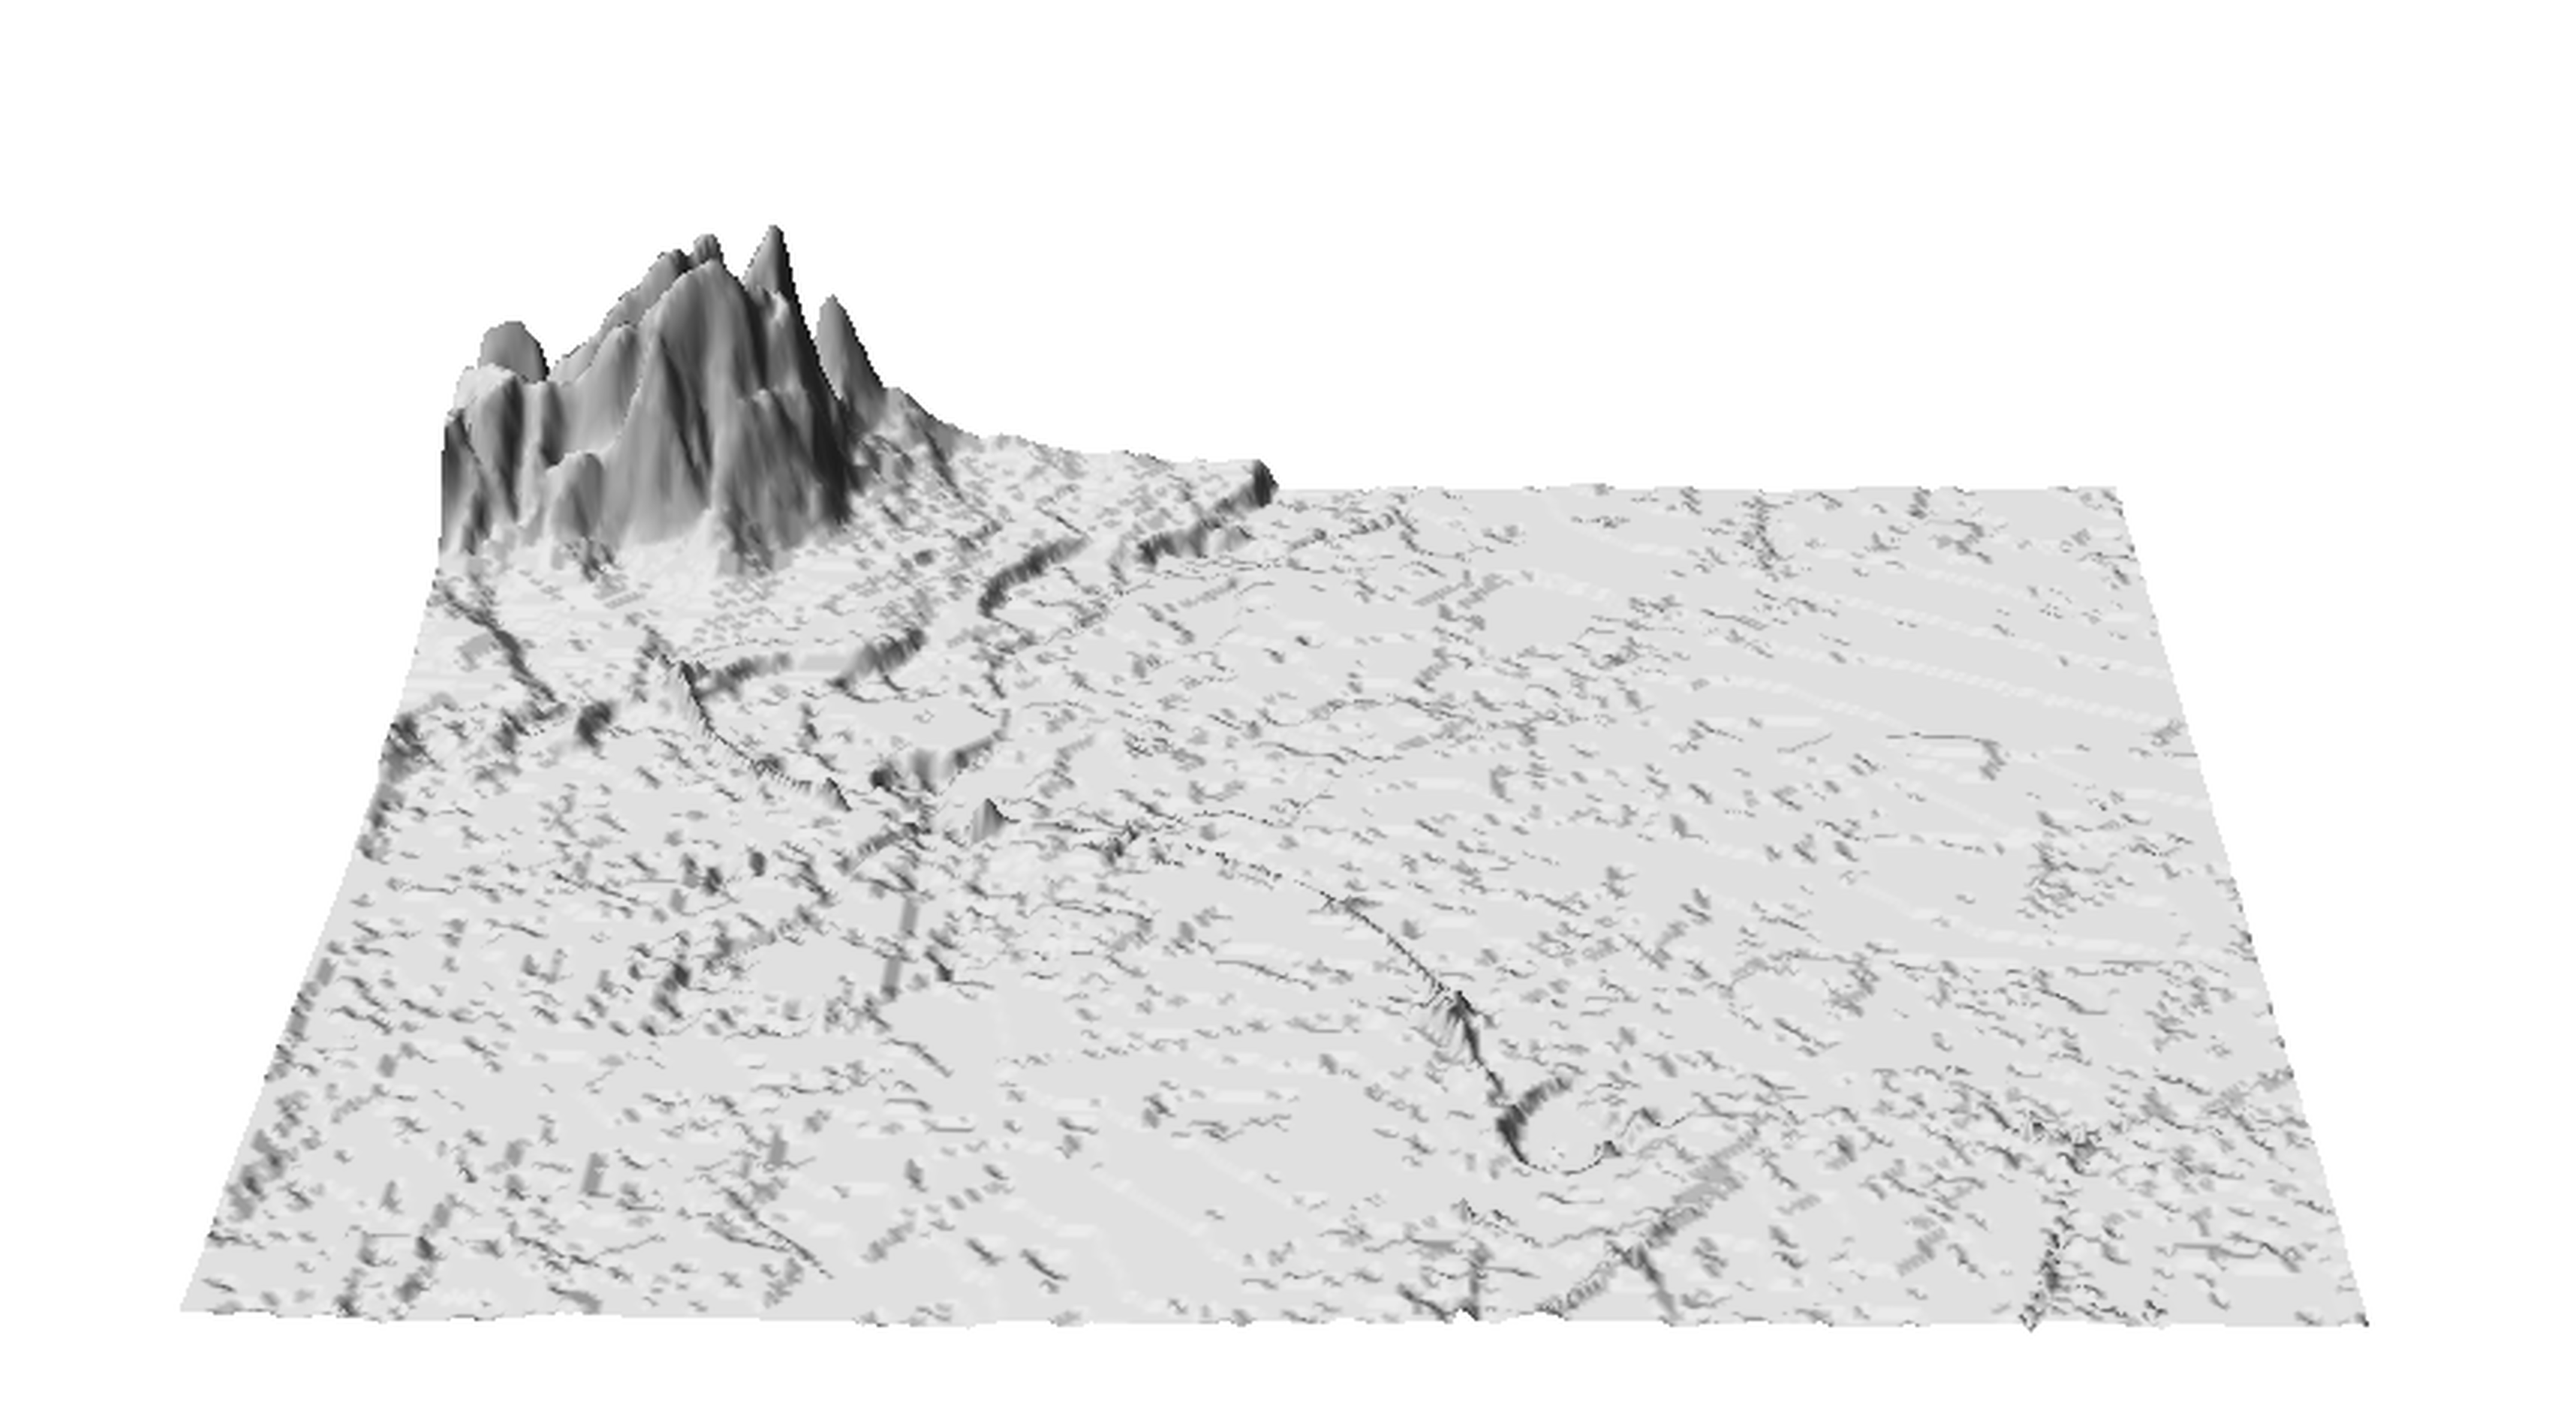
\includegraphics[width=1\columnwidth]{\lyxdot \lyxdot /tun_par/doc/img/terrain_MS}

\caption{Terrain profile of the test network Net$_{8}$, dominated by a flat
agricultural area. \label{fig:05-Terrain_profile_for_Net8}}
%
\end{minipage}\hfill{}%
\begin{minipage}[t]{0.49\textwidth}%
\centering

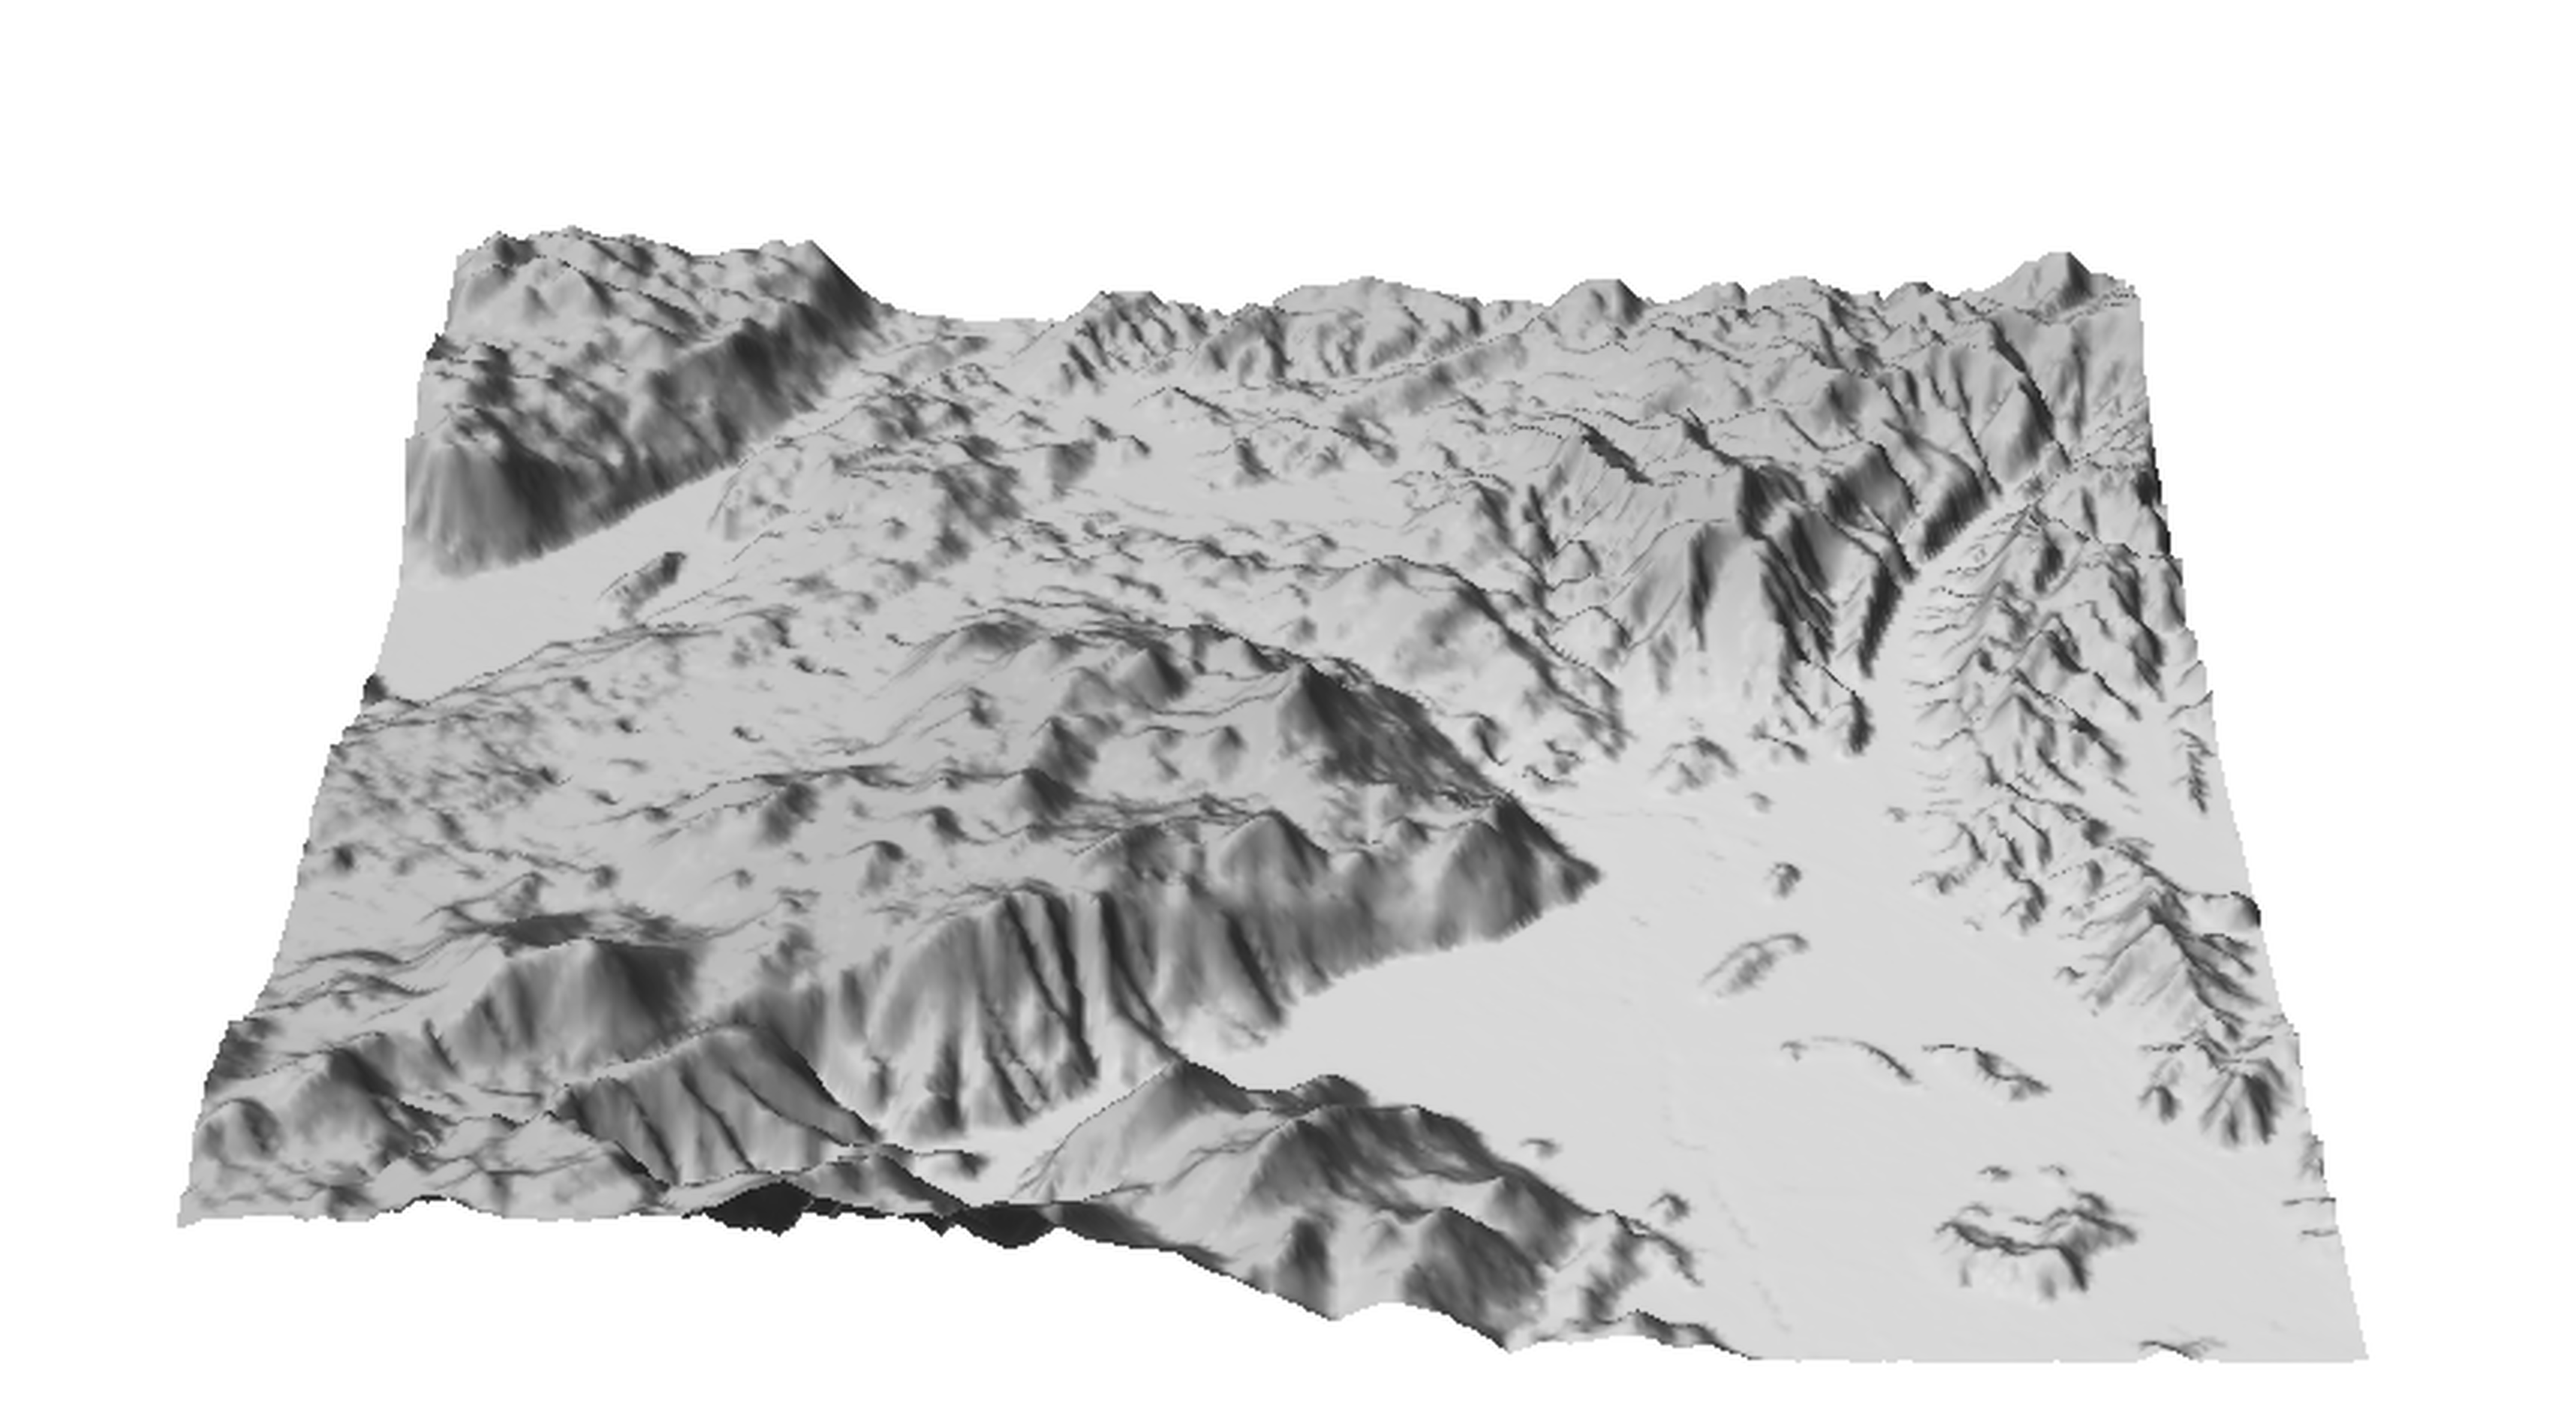
\includegraphics[width=1\columnwidth]{\lyxdot \lyxdot /tun_par/doc/img/terrain_HI}

\caption{Terrain profile of the test network Net$_{10}$, dominated by forested
hills. \label{fig:05-Terrain_profile_for_Net10}}
%
\end{minipage}
\end{figure}


In the following, the default parameters of the radio-propagation
model correspond to the values provided by the engineers of the Radio
Network department at Telekom Slovenije, d.d.

\bigskip{}


The simulations were carried out on several computing nodes of the
previously presented DEGIMA cluster~\cite{Hamada_Cluster_of_GPUs:2010}
at the NACC of the Nagasaki University in Japan (see Section~\ref{sec:04-Simulations}).
Groups of 3, 4, and 34 nodes were used for executing the simulations
of the different problem instances, i.e., Net$_{8}$, Net$_{9}$ and
Net$_{10}$, respectively.


\subsection{Results \label{sub:05-Least_squares_results}}

The results of applying the linear least-squares method to fit the
parameters of the radio-propagation model to a set of field measurements
are presented in this section. Bar charts were prepared to show the
cumulative distribution of the absolute error between the radio-propagation
prediction and the field measurements (see Figures~\ref{fig:05-Error_distribution_for_Net8},
\ref{fig:05-Error_distribution_for_Net9}, and \ref{fig:05-Error_distribution_for_Net10}).
Each bar represents an open interval, expressed in dB, denoting the
proportion of points that deviate from the prediction in the given
number of dB. For example, in Figure~\ref{fig:05-Error_distribution_for_Net8}~(a),
it can be observed that the proportion of predicted points differing
from the field measurements in 35~dB or more is around 16~\%, whereas
the proportion of points differing in less than 5~dB is 10~\%. These
values correspond to the test network Net$_{8}$, before applying
the model-parameter fitting. For comparison, in Figure~\ref{fig:05-Error_distribution_for_Net8}~(b),
the absolute-error distribution for the same test network is given,
but with the model parameters fitted to the available field measurements.
Notice how the proportions describing the biggest deviation have dropped
to under 5~\% (35~dB and more), and to less than 6~\% (30~dB to
35~dB), respectively. Moreover, it is clear how all proportions improved,
raising the bars towards the left-hand side of the chart and lowering
them on the right-hand side.

The error distributions of the radio-propagation prediction for test
network Net$_{9}$ using the default parameters and the fitted ones
are given in Figures~\ref{fig:05-Error_distribution_for_Net9}~(a)
and \ref{fig:05-Error_distribution_for_Net9}~(b), respectively.
In this case, the improvement is even more significant than for the
previous test network, clearly showing that the tuned propagation
model represents the local radio-propagation conditions more accurately
than the default parameter set.

For the last test network, Net$_{10}$, the error distributions are
depicted in Figure~\ref{fig:05-Error_distribution_for_Net10}~(a)
using the default parameters, and Figure~\ref{fig:05-Error_distribution_for_Net10}~(b)
for the tuned ones. Similar to the test network Net$_{8}$, it can
be clearly seen how the proportions of highest error deviations have
been lowered with respect to those with lower deviation values. 

The overall results confirm that fitting the parameters of the radio-propagation
model to the field measurements of each network cell significantly
improves the quality of the calculated radio-propagation predictions.
Indeed, since the default parameters were provided by the radio engineers
after following a traditional approach for the whole network, it can
be concluded that the automated-fitting method is not only simpler
and faster, but also superior in terms of solution quality.

However, it is important to note the particular reasons behind the
considerable better results for Net$_{9}$, when compared to those
of Net$_{8}$ and Net$_{10}$. Clearly, the relative quantity of the
available field measurements directly affects the quality of the calculated
results. Therefore, the least squares approximation is rougher and
less precise for the networks where the field-measurement proportion
is lower. See Table~\ref{tab:05-Test_network_properties} for a reference
of the field-measurement proportions with respect to the area surface
of each test network. Similar findings were confirmed by other authors,
who worked on the adjustment of radio-propagation models to different
environments~\cite{Huang_Online_propagation_model_correction_based_on_PSO_algorithm_in_LTE_SON_system:2012}.
For the sake of completeness, it is worth pointing out that some researchers
have already started working on different ways on how to improve this
aspect~\cite{Neuland_Influence_of_Different_Factors_on_X_Map_Estimation_in_LTE:2011,Neuland_Influence_of_positioning_error_on_X_Map_estimation_in_LTE:2011}.

\begin{figure}
\centering

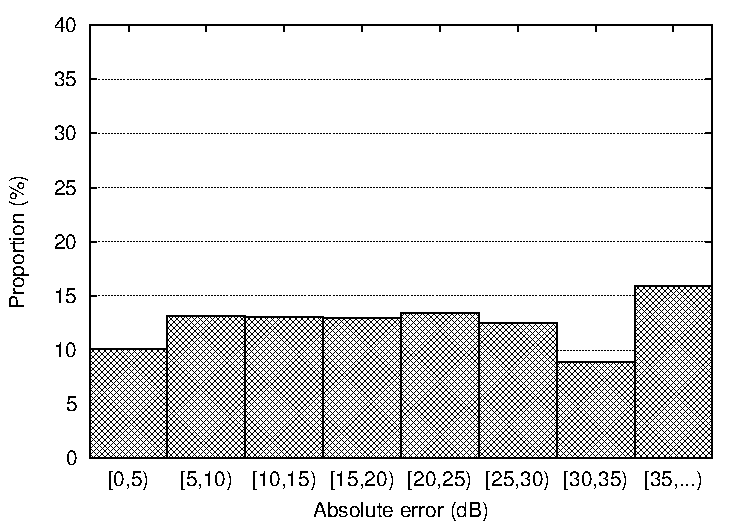
\includegraphics[width=0.47\textwidth]{\lyxdot \lyxdot /tun_par/doc/img/error_distribution-MS-def_params}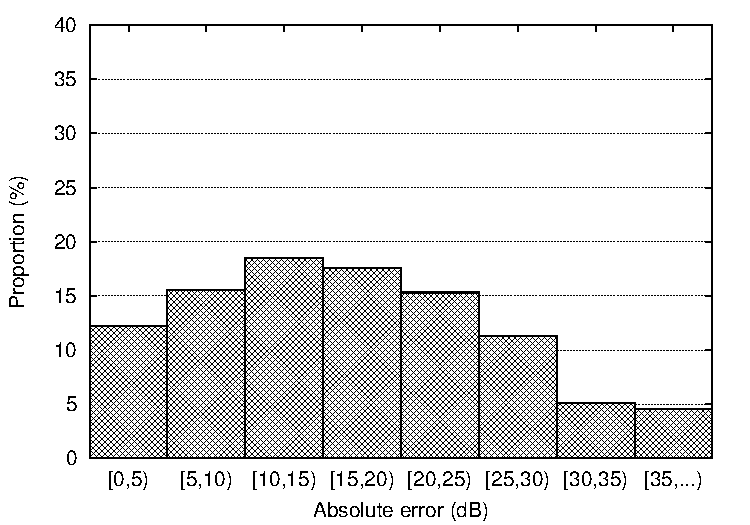
\includegraphics[width=0.47\textwidth]{\lyxdot \lyxdot /tun_par/doc/img/error_distribution-MS-opt_params}\\\hspace{0.4cm}(a)\hspace{6.7cm}(b)

\caption{Error distribution of the radio prediction for network Net$_{8}$:
(a) with default parameter values, and (b) with fitted parameter values.\label{fig:05-Error_distribution_for_Net8}}
\end{figure}


\begin{figure}[h]
\centering

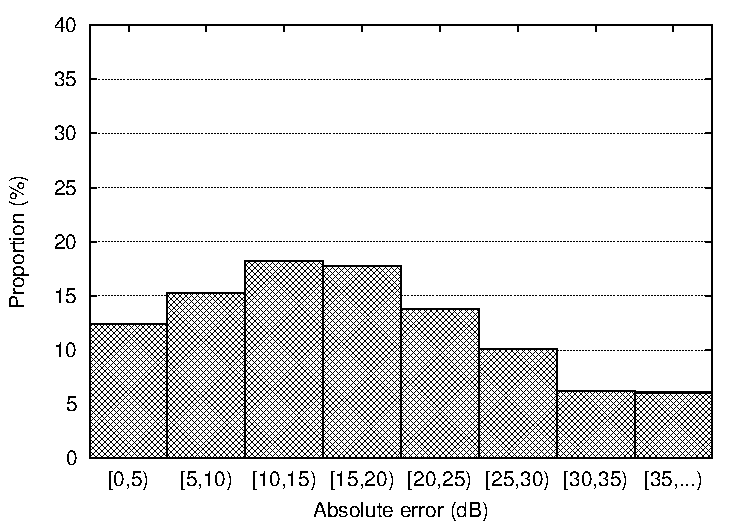
\includegraphics[width=0.47\textwidth]{\lyxdot \lyxdot /tun_par/doc/img/error_distribution-LJ-opt_params}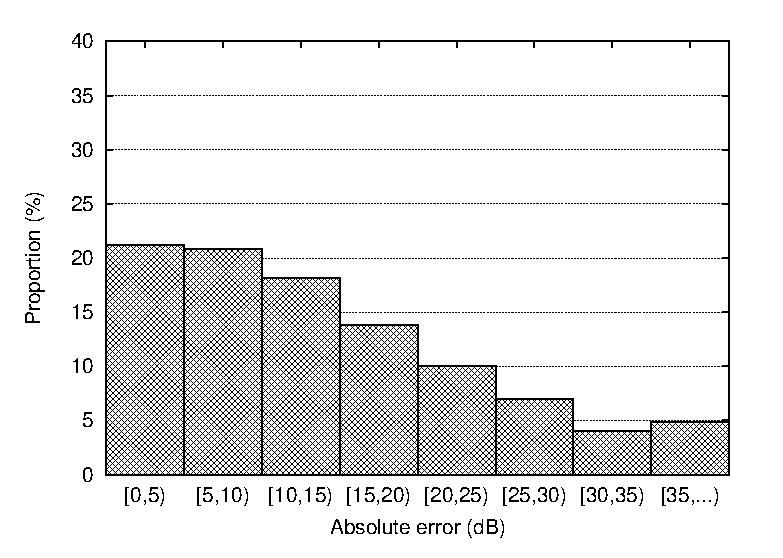
\includegraphics[width=0.47\textwidth]{\lyxdot \lyxdot /tun_par/doc/img/error_distribution-LJ-def_params}\\\hspace{0.4cm}(a)\hspace{6.7cm}(b)

\caption{Error distribution of the radio prediction for network Net$_{9}$:
(a) with default parameter values, and (b) with fitted parameter values.\label{fig:05-Error_distribution_for_Net9}}
\end{figure}


\begin{figure}[H]
\centering

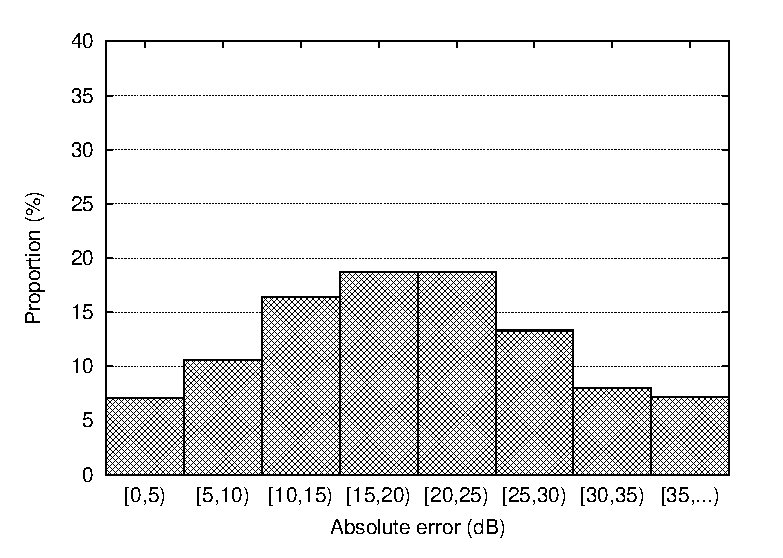
\includegraphics[width=0.47\textwidth]{\lyxdot \lyxdot /tun_par/doc/img/error_distribution-HI-def_params}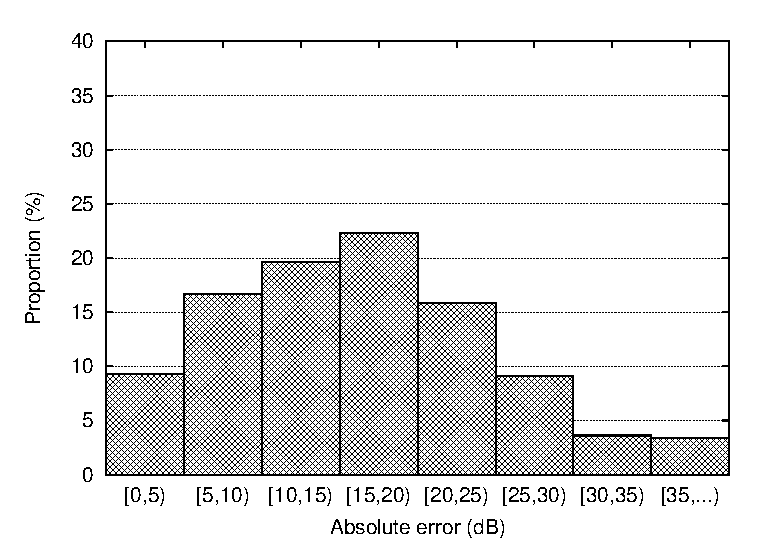
\includegraphics[width=0.47\textwidth]{\lyxdot \lyxdot /tun_par/doc/img/error_distribution-HI-opt_params}\\\hspace{0.4cm}(a)\hspace{6.7cm}(b)

\caption{Error distribution of the radio prediction for network Net$_{10}$:
(a) with default parameter values, and (b) with fitted parameter values.\label{fig:05-Error_distribution_for_Net10}}
\end{figure}



\section{Clutter optimization \label{sec:05-Clutter_optimization}}

In order to further improve the accuracy of the radio-prediction calculation
over a given regional environment, the signal losses due to clutter
are optimized in this section.

As it was mentioned before, there are several reasons for the predicted
signal-loss values to be inaccurate. The seasonal changes are among
them, like tree foliage and snow. Also, changes related to urban development,
like demolition or construction of buildings and parks, and different
kinds of forests or agricultural areas, etc. These changes are only
noticeable through regular updates of accurate land-usage data. However,
in the short term, updates are only available in the form of feedback
by means of field-measurement campaigns.

In the following, a metaheuristic algorithm is used to optimize the
clutter losses of several regions within a target radio network. This
is done over groups of network cells within different regions of the
target network, e.g., agricultural, urban or hilly. In terms of coverage
planning, a regional classification of the signal losses due to clutter
improves the accuracy of the radio-coverage prediction.

In contrast to the parameter tuning of the mathematical model presented
in Section~\ref{sec:05-Parameter_tuning_radio-propagation_model},
an analytical approach is not used for tackling this problem. Instead,
the DASA metaheuristic algorithm is the tool of choice for optimizing
the clutter losses.

There are several reasons for choosing the DASA as the optimization
algorithm in the context of this problem. First, the benefits of metaheuristic
algorithms for solving optimization problems, particularly in the
context of radio networks, was demonstrated by several authors in
general~\cite{Benedicic_Balancing_downlink_uplink_soft_handover_areas_in_UMTS_networks:2012,Garcia-Lozano_Metaheuristic_procedure_to_optimize_transmission_delays_in_DVB-T_single_frequency_networks:2011,Huang_Online_propagation_model_correction_based_on_PSO_algorithm_in_LTE_SON_system:2012,Malla_Energy_efficient_resource_allocation_in_OFDMA_networks_using_ant_colony_optimization:2012},
and in this thesis in particular (see Chapters~\ref{chap:02-Optimization_of_radio_networks},
\ref{chap:06-Experimental-evaluation-the-service-coverage-problem}
and~\ref{chap:07-Experimental-evaluation-the-SHO-alignment-problem}).
Second, in~\cite{korosec2010_DASA}, the authors validated the suitability
of the algorithm for solving numerical-optimization problems.


\subsection{Optimization objective \label{sub:Optimization-objective}}

The optimization objective consists of adjusting the loss values of
the different clutter categories, i.e., $\mathrm{L}{}_{\mathrm{CLUT}}(d_{(x,y)})$
as used in Equation~(\ref{eq:04-Hata_pathloss}), according to a
set of field measurements of a given geographical region. The same
three data sets used in Section~\ref{sub:05-Simulations} were used
for the clutter-optimization problem: the first for Net$_{8}$, the
second for Net$_{9}$, and the third for Net$_{10}$. Each region
was independently optimized, so that the radio-propagation predictions
of each set of network cells minimized the mean-squared error against
the field measurements, i.e.:

\begin{equation}
\min f_{\mathrm{clut}}=\sum_{i=1}^{m_{c}}\frac{(p_{c}-\mathrm{L}{}_{c}(i,\vec{\beta_{c}^{*}})-fm_{i})^{2}}{m_{C}}\;\forall c\in C,\label{eq:05-Mean-squared_error}
\end{equation}


\noindent where $f_{\mathrm{clut}}$ is the optimization objective
to be minimized in each of the three regions, $p_{c}$ is the transmit
power of cell $c$, $fm_{i}$ is the $i$-th field measurement of
cell $c$, the set of which has cardinality $m_{c}$, and $m_{C}$
is the number of field measurements of all the cells of a given network.
Similar to the least-squares approach, $\mathrm{L}{}_{c}(i,\vec{\beta_{c}^{*}})$
represents the path loss of cell $c$ at the same geographical point
of the $i$-th field measurement, and $\vec{\beta_{c}^{*}}$ denotes
the fitted parameter vector of the prediction model for cell $c$.

For a reference of the different clutter categories used by the radio-propagation
model, see Table~\ref{tab:05-Clutter_categories}.


\subsection{Differential ant-stigmergy algorithm}

The chosen optimization algorithm for the clutter-optimization problem
is the DASA (see Section~\ref{sub:02-DASA}). The mapping between
the clutter-optimization problem and DASA is as follows:

\begin{equation}
X_{a}=\left\{ x_{0},x_{1},\ldots,x_{i},\ldots,x_{11}\right\} ,\label{eq:DASA-problem_mapping}
\end{equation}


\noindent where $X_{a}$ is the solution vector of ant $a$ during
the minimization process, and $x_{i}$ represents the $i$-th clutter
category within a given region or network. At the end of every iteration,
and after all the ants have created solutions, they are evaluated
to establish if any of them is better than the best solution found
so far.


\subsection{Simulations}

In this case, one simulation round consisted of multiple iterations
of several steps. An iteration begins by generating a solution vector
for each of the ants in the DASA colony. The following step involves
the parallel evaluation of the solution vector carried by an ant,
i.e., one radio-propagation prediction per worker process. The final
step consists in calculating the objective-function value, as defined
in Equation~(\ref{eq:05-Mean-squared_error}), before sending it
back to the master process for the DASA to generate the next set of
solutions. Figure~\ref{fig:05-PRATO_architecture_optimization} depicts
the way PRATO performs the parallel objective-function evaluation
over the worker processes, while the optimization algorithm runs on
the master process.

\begin{figure}
\centering

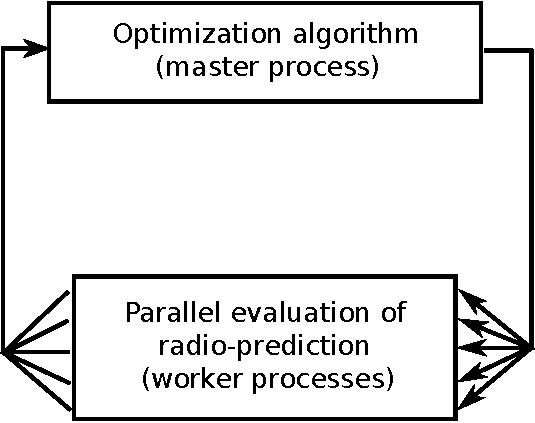
\includegraphics[width=0.4\textwidth]{05-framework_parameter_tuning/img/architecture}

\caption{\textit{\emph{Architecture and data flow of PRATO during the clutter-optimization
phase. The optimization algorithm runs on the master process, while
the radio-propagation predictions of the involved network cells run
in parallel over several worker processes. \label{fig:05-PRATO_architecture_optimization}}}}
\end{figure}


As opposed to the least-squares case, a much larger number of evaluations
is needed for this kind of optimization. Therefore, it is essential
to exploit the parallel nature of the framework in order to simultaneously
evaluate the radio-coverage prediction of multiple cells. Otherwise,
a metaheuristic approach would not be feasible, due to the computational
time required to reach a reasonable solution.

The default clutter-loss values (expressed in dB) for each clutter
category, which are listed in the second column of Table~\ref{tab:05-Clutter_optimization_solutions},
were provided by the radio experts of the Radio Network department
at Telekom Slovenije, d.d. These values were empirically calculated
using a classic (i.e., manual) approach, the results of which are
regularly loaded into a commercial radio-planning application in order
to validate the radio coverage at a network-wide level. The radio
experts also suggested limiting the optimized clutter-loss values
to a maximum of 40~dB.

The stopping criteria for the optimization runs was set by limiting
the maximum number of objective-function evaluations. In this sense,
the limits for Net$_{8}$ and Net$_{10}$ were set the 200, whereas
for Net$_{9}$ the value was 500, since this network contains the
largest number of cells. Overall, the framework completed 48,000 objective-function
evaluations, i.e., 576,000 radio-coverage predictions for Net$_{8}$
and 288,000 for Net$_{10}$, whereas for Net$_{9}$, the number of
objective-function evaluations was 120,000, for a total of 15,600,000
radio-coverage predictions.

Regarding the parameters that control the behavior of the DASA, they
were set to the following values after some trial-optimization runs:
\begin{itemize}
\item $m=240$, the number of ants;
\item $b=10,$ the discrete base;
\item $\rho=0.2$, the pheromone dispersion factor;
\item $s_{+}=0.01$, the global scale-increasing factor;
\item $s_{-}=0.01$, the global scale-decreasing factor; and 
\item $\epsilon=1.0^{-2}$, the maximum parameter precision.
\end{itemize}
The trial runs consisted in doubling $m$ from 15 to 480, and verifying
the convergence profile and best solution found. The values of the
other parameters were left unchanged.


\subsection{Results}

\begin{table}
\centering

\caption{Clutter-category losses after the optimization. The default losses
for each clutter category are given along the solutions for each of
the test networks. All values are expressed in dB. \label{tab:05-Clutter_optimization_solutions}}


{\small{}}%
\begin{tabular}{ccccc}
\hline 
{\small{Clutter category}} & {\small{Default}} & {\small{Net$_{8}$}} & {\small{Net$_{9}$}} & {\small{Net$_{10}$}}\tabularnewline
\hline 
{\small{0}} & {\small{5.0}} & {\small{13.71}} & {\small{11.30}} & {\small{17.90}}\tabularnewline
{\small{1}} & {\small{15.0}} & {\small{12.39}} & {\small{16.67}} & {\small{-}}\tabularnewline
{\small{2}} & {\small{13.0}} & {\small{16.04}} & {\small{17.04}} & {\small{15.69}}\tabularnewline
{\small{3}} & {\small{28.0}} & {\small{19.59}} & {\small{18.01}} & {\small{23.00}}\tabularnewline
{\small{4}} & {\small{12.0}} & {\small{11.48}} & {\small{9.71}} & {\small{10.80}}\tabularnewline
{\small{5}} & {\small{20.0}} & {\small{16.26}} & {\small{11.62}} & {\small{16.26}}\tabularnewline
{\small{6}} & {\small{15.0}} & {\small{-}} & {\small{-}} & {\small{-}}\tabularnewline
{\small{7}} & {\small{8.0}} & {\small{-}} & {\small{13.49}} & {\small{-}}\tabularnewline
{\small{8}} & {\small{5.0}} & {\small{-}} & {\small{13.50}} & {\small{-}}\tabularnewline
{\small{9}} & {\small{1.0}} & {\small{17.50}} & {\small{5.60}} & {\small{-}}\tabularnewline
{\small{10}} & {\small{20.0}} & {\small{8.26}} & {\small{16.75}} & {\small{16.63}}\tabularnewline
{\small{11 }} & {\small{8.0}} & {\small{-}} & {\small{18.93}} & {\small{-}}\tabularnewline
\hline 
\end{tabular}
\end{table}


The results achieved by the optimization process are shown in Table~\ref{tab:05-Clutter_optimization_solutions}.
The solutions are given for each of the test networks, along with
the empirically-calculated (default) loss values. Hyphens represent
clutter categories for which there were no field measurements available.
Consequently, it was not possible to evaluate the objective-function
for them.

The optimized loss for the first clutter category, 0, representing
urban area without buildings, is larger than the default value in
all three networks. This may be attributed to the fact that these
areas are not completely open, mostly surrounded by forests (Net$_{8}$
and Net$_{10}$) and buildings of different sizes (Net$_{9}$). As
for the category 1, representing suburban area, the value for Net$_{8}$
is lower than the default one, mainly because this network is deployed
over a predominant agricultural area, i.e., suburban areas are less
dense here. On the other hand, the value for Net$_{9}$ is larger,
indicating a building density above the average, whereas for Net$_{10}$,
the value could not be calculated due to the lack of measurements.
For the category 2, representing urban area, the optimized values
are above the default ones, clearly showing an underestimation of
the manual approach. However, there is a relation among the clutter
losses that corresponds to the population density in each of the regions,
being Net$_{10}$ the less dense urban area among the three networks.
The optimized values of the category 3, representing dense urban area,
are lower than the default ones. This indicates that the dense urban
areas in these regions have a lower density than the average case.
Representing the agricultural area, the category 4 gets a value very
close to the default one for Net$_{8}$ and Net$_{10}$, whereas for
Net$_{9}$ the value is lower, indicating that this type of land is
mostly open near the city, e.g., without plantations. As for the category
5, representing forests, the results correspond with the type of forest
that dominates each of the test-network regions. Namely, Net$_{8}$
and Net$_{10}$ are dominated by dense forests presenting leave foliage,
whereas in Net$_{9}$ the forests are mostly coniferous and more sparse.
Keeping most of the default loss values for the categories 6, 7 and
8, the results of the next category, 9, representing water, indicate
creeks and rivers in these areas are almost entirely surrounded by
forests (Net$_{8}$) or buildings (Net$_{9}$), since none of the
regions lays by the sea. As for the industrial area, denoted by the
clutter category 10, lower loss values than the empirically-calculated
defaults appear. This indicates the presence of sparse industrial
buildings in Net$_{8}$, and a higher density of mostly commercial
buildings for Net$_{9}$ and Net$_{10}$. The last clutter category,
11, could not be calculated for Net$_{8}$ and Net$_{10}$ due to
the lack of field measurements.

Notice that the relation among the different clutter categories is
correctly kept for the three test networks. For example, it can be
observed that the clutter loss for dense urban area (category 3) is
higher than the values of the urban area (category 2), as well as
of the agricultural area (category 4). Hence, the results reflect
physically feasible losses, despite the higher deviation from the
default losses shown by the category 2, and the lower deviation for
the category 3, again with respect to the default losses. Such relations
hold for different categories of all three test networks, strongly
suggesting the correctness of the applied optimization approach and
the evaluation methodology used. Consequently, it can be confirmed
that the combination of PRATO and a metaheuristic algorithm is applicable
for performing the automatic adjustment of clutter losses, since it
is capable of reflecting the physical phenomena appearing in real-world
conditions and improving the quality of radio-propagation predictions
for three, geographically different, radio-network instances.

\bigskip{}


Similar to Section~\ref{sub:05-Least_squares_results}, bar charts
show the cumulative distribution of the absolute error between the
signal-propagation prediction and the field measurements (see Figures~\ref{fig:05-Clutter_error_distribution_for_Net8},
\ref{fig:05-Clutter_error_distribution_for_Net9}, and \ref{fig:05-Clutter_error_distribution_for_Net10}).
Figure~\ref{fig:05-Clutter_error_distribution_for_Net8}~(a) depicts
the error distribution of the prediction for test network Net$_{8}$
using the fitted model parameters, whereas Figure~\ref{fig:05-Clutter_error_distribution_for_Net8}~(b)
shows the absolute-error distribution for the same test network, but
using the optimized clutter losses (see Table~\ref{tab:05-Clutter_optimization_solutions},
column Net$_{8}$). Notice how the error distributions show an improvement
when the optimized clutter losses are used, lowering the biggest (right-most)
deviations even further.

The error distributions of the radio-propagation predictions for test
network Net$_{9}$ using fitted parameters and default clutter losses,
and fitted parameters with optimized clutter losses, are shown in
Figures~\ref{fig:05-Clutter_error_distribution_for_Net9}~(a) and
\ref{fig:05-Clutter_error_distribution_for_Net9}~(b), respectively.
Similar to Net$_{8}$, the improvement appears in the biggest deviations,
since their values are lower than when using the default clutter losses.

\begin{figure}[h]
\centering

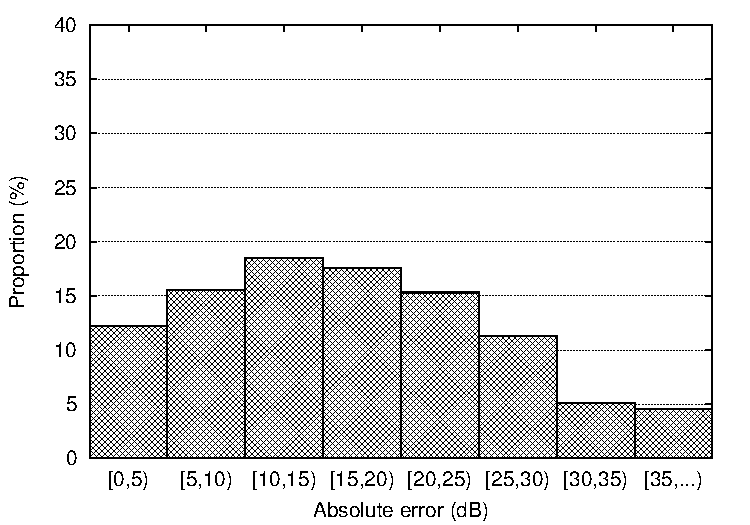
\includegraphics[width=0.47\textwidth]{\lyxdot \lyxdot /tun_par/doc/img/error_distribution-MS-opt_params}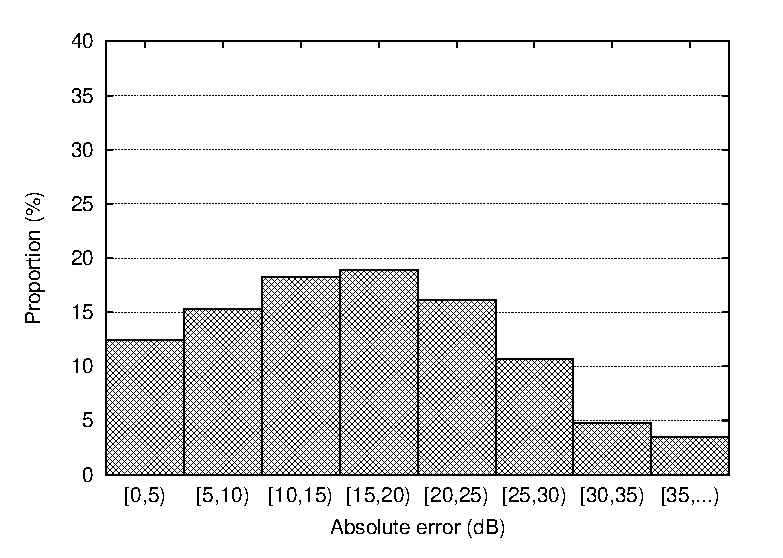
\includegraphics[width=0.47\textwidth]{\lyxdot \lyxdot /tun_par/doc/img/error_distribution-MS-opt_clutter}\\\hspace{0.4cm}(a)\hspace{6.7cm}(b)

\caption{Error distribution of the radio prediction for network Net$_{8}$:
(a) with fitted parameter values and default clutter losses, and (b)
with fitted parameter values and optimized clutter losses.\label{fig:05-Clutter_error_distribution_for_Net8}}
\end{figure}


\begin{figure}[h]
\centering

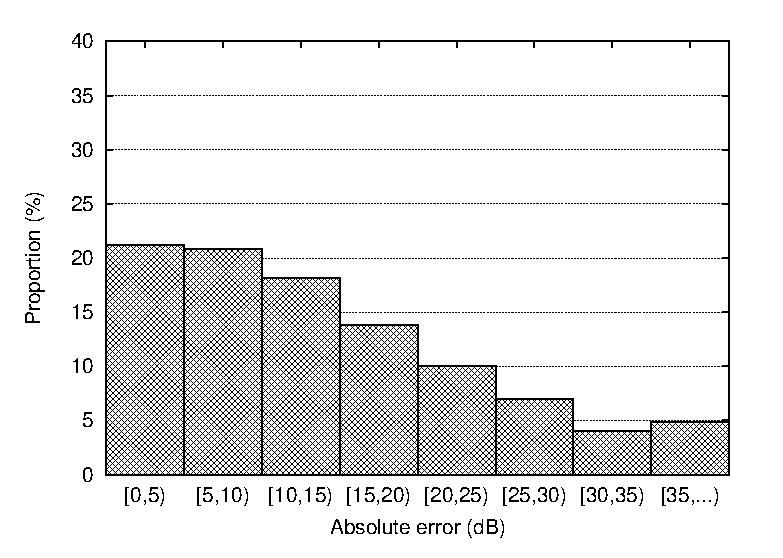
\includegraphics[width=0.47\textwidth]{\lyxdot \lyxdot /tun_par/doc/img/error_distribution-LJ-def_params}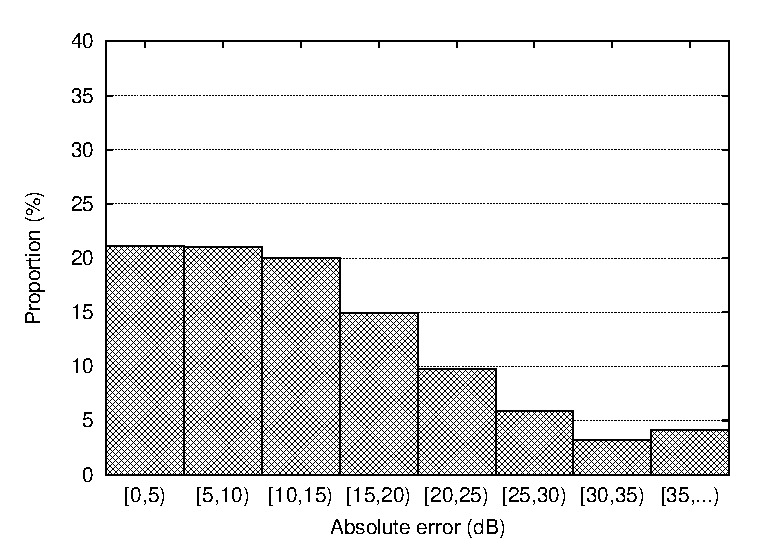
\includegraphics[width=0.47\textwidth]{\lyxdot \lyxdot /tun_par/doc/img/error_distribution-LJ-opt_clutter}\\\hspace{0.4cm}(a)\hspace{6.7cm}(b)

\caption{Error distribution of the radio prediction for network Net$_{9}$:
(a) with fitted parameter values and default clutter losses, and (b)
with fitted parameter values and optimized clutter losses.\label{fig:05-Clutter_error_distribution_for_Net9}}
\end{figure}


\begin{figure}[H]
\centering

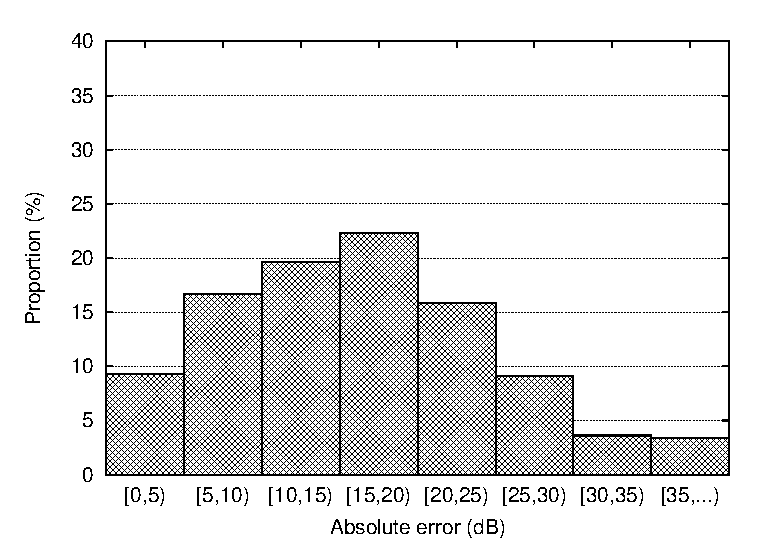
\includegraphics[width=0.47\textwidth]{\lyxdot \lyxdot /tun_par/doc/img/error_distribution-HI-opt_params}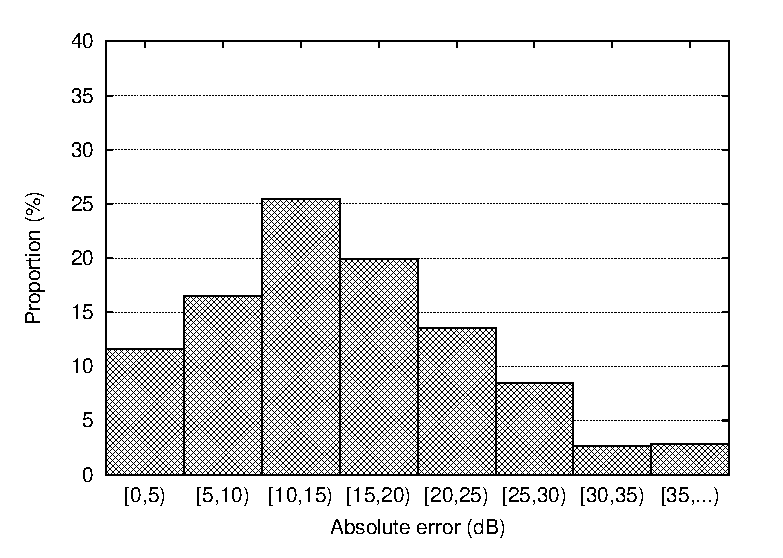
\includegraphics[width=0.47\textwidth]{\lyxdot \lyxdot /tun_par/doc/img/error_distribution-HI-opt_clutter}\\\hspace{0.4cm}(a)\hspace{6.7cm}(b)

\caption{Error distribution of the radio prediction for network Net$_{10}$:
(a) with fitted parameter values and default clutter losses, and (b)
with fitted parameter values and optimized clutter losses.\label{fig:05-Clutter_error_distribution_for_Net10}}
\end{figure}


For the last test network, Net$_{10}$, the error distributions are
depicted in Figure~\ref{fig:05-Clutter_error_distribution_for_Net10}~(a)
using the default clutter losses, and Figure~\ref{fig:05-Clutter_error_distribution_for_Net10}~(b)
for the optimized ones. Again, the fitted model parameters were used
for both simulation sets. In this case, a more significant improvement
than for the other two networks appears, clearly showing the favorable
effect of the optimization process. Moreover, this result suggests
that some of the default clutter losses considerably fail in representing
the actual physical conditions in the geographical region of this
network.

Overall, the presented results confirm that the optimization of clutter
losses with respect to field measurements improves the quality of
the calculated radio-propagation predictions. Considering the default
clutter losses were empirically calculated by the radio engineers
for the whole network, the convenience of the automated optimization
procedure is clear. Indeed, these advantages are a consequence of
a simpler method that automatically delivers radio-predictions of
superior quality, thus accurately representing the physical properties
of a given environment.

\begin{table}
\centering

\caption{Statistical analysis of the solutions for the clutter-optimization
problem. All values are expressed in dB. The corresponding box plots
are depicted in Figure~\ref{fig:05-Statistical_analysis_boxplots}.
\label{tab:05-Statistical_analysis_of_solutions}}


{\scriptsize{}}%
\begin{tabular}{>{\centering}p{0.2cm}cccc>{\centering}p{0.75cm}cccc>{\centering}p{0.75cm}cccc>{\centering}p{0.75cm}}
\cline{3-16} 
 &  &  & \multicolumn{2}{c}{{\scriptsize{Net$_{8}$}}} &  &  &  & \multicolumn{2}{c}{{\scriptsize{Net$_{9}$}}} &  &  &  & \multicolumn{2}{c}{{\scriptsize{Net$_{10}$}}} & \tabularnewline
\hline 
{\scriptsize{Cat.}} &  & {\scriptsize{Min}} & {\scriptsize{Max}} & {\scriptsize{Avg}} & {\scriptsize{St.dev.}} &  & {\scriptsize{Min}} & {\scriptsize{Max}} & {\scriptsize{Avg}} & {\scriptsize{St.dev.}} &  & {\scriptsize{Min}} & {\scriptsize{Max}} & {\scriptsize{Avg}} & {\scriptsize{St.dev.}}\tabularnewline
\hline 
{\scriptsize{0}} &  & {\scriptsize{13.36}} & {\scriptsize{13.97}} & {\scriptsize{13.71}} & {\scriptsize{0.15}} &  & {\scriptsize{11.22}} & {\scriptsize{11.40}} & {\scriptsize{11.30}} & {\scriptsize{0.04}} &  & {\scriptsize{17.72}} & {\scriptsize{17.85}} & {\scriptsize{17.90}} & {\scriptsize{0.07}}\tabularnewline
\cline{1-6} \cline{8-11} \cline{13-16} 
{\scriptsize{1}} &  & {\scriptsize{-}} & {\scriptsize{-}} & {\scriptsize{-}} & {\scriptsize{-}} &  & {\scriptsize{14.25}} & {\scriptsize{19.20}} & {\scriptsize{16.67}} & {\scriptsize{1.87}} &  & {\scriptsize{-}} & {\scriptsize{-}} & {\scriptsize{-}} & {\scriptsize{-}}\tabularnewline
\cline{1-6} \cline{8-11} \cline{13-16} 
{\scriptsize{2}} &  & {\scriptsize{15.84}} & {\scriptsize{16.21}} & {\scriptsize{16.04}} & {\scriptsize{0.08}} &  & {\scriptsize{16.99}} & {\scriptsize{17.11}} & {\scriptsize{17.04}} & {\scriptsize{0.03}} &  & {\scriptsize{15.64}} & {\scriptsize{15.72}} & {\scriptsize{15.69}} & {\scriptsize{0.03}}\tabularnewline
\cline{1-6} \cline{8-11} \cline{13-16} 
{\scriptsize{3}} &  & {\scriptsize{19.15}} & {\scriptsize{20.07}} & {\scriptsize{19.59}} & {\scriptsize{0.25}} &  & {\scriptsize{17.95}} & {\scriptsize{18.12}} & {\scriptsize{18.01}} & {\scriptsize{0.04}} &  & {\scriptsize{22.68}} & {\scriptsize{23.20}} & {\scriptsize{23.00}} & {\scriptsize{0.16}}\tabularnewline
\cline{1-6} \cline{8-11} \cline{13-16} 
{\scriptsize{4}} &  & {\scriptsize{11.35}} & {\scriptsize{11.62}} & {\scriptsize{11.48}} & {\scriptsize{0.05}} &  & {\scriptsize{9.63}} & {\scriptsize{9.77}} & {\scriptsize{9.71}} & {\scriptsize{0.03}} &  & {\scriptsize{10.73}} & {\scriptsize{10.84}} & {\scriptsize{10.80}} & {\scriptsize{0.03}}\tabularnewline
\cline{1-6} \cline{8-11} \cline{13-16} 
{\scriptsize{5}} &  & {\scriptsize{16.00}} & {\scriptsize{16.54}} & {\scriptsize{16.26}} & {\scriptsize{0.14}} &  & {\scriptsize{11.45}} & {\scriptsize{11.80}} & {\scriptsize{11.62}} & {\scriptsize{0.08}} &  & {\scriptsize{16.19}} & {\scriptsize{16.30}} & {\scriptsize{16.26}} & {\scriptsize{0.04}}\tabularnewline
\cline{1-6} \cline{8-11} \cline{13-16} 
{\scriptsize{6}} &  & {\scriptsize{-}} & {\scriptsize{-}} & {\scriptsize{-}} & {\scriptsize{-}} &  & {\scriptsize{-}} & {\scriptsize{-}} & {\scriptsize{-}} & {\scriptsize{-}} &  & {\scriptsize{-}} & {\scriptsize{-}} & {\scriptsize{-}} & {\scriptsize{-}}\tabularnewline
\cline{1-6} \cline{8-11} \cline{13-16} 
{\scriptsize{7}} &  & {\scriptsize{-}} & {\scriptsize{-}} & {\scriptsize{-}} & {\scriptsize{-}} &  & {\scriptsize{12.71}} & {\scriptsize{14.52}} & {\scriptsize{13.49}} & {\scriptsize{0.39}} &  & {\scriptsize{-}} & {\scriptsize{-}} & {\scriptsize{-}} & {\scriptsize{-}}\tabularnewline
\cline{1-6} \cline{8-11} \cline{13-16} 
{\scriptsize{8}} &  & {\scriptsize{-}} & {\scriptsize{-}} & {\scriptsize{-}} & {\scriptsize{-}} &  & {\scriptsize{12.25}} & {\scriptsize{15.79}} & {\scriptsize{13.50}} & {\scriptsize{0.83}} &  & {\scriptsize{-}} & {\scriptsize{-}} & {\scriptsize{-}} & {\scriptsize{-}}\tabularnewline
\cline{1-6} \cline{8-11} \cline{13-16} 
{\scriptsize{9}} &  & {\scriptsize{16.07}} & {\scriptsize{18.80}} & {\scriptsize{17.50}} & {\scriptsize{0.83}} &  & {\scriptsize{4.67}} & {\scriptsize{6.26}} & {\scriptsize{5.60}} & {\scriptsize{0.35}} &  & {\scriptsize{-}} & {\scriptsize{-}} & {\scriptsize{-}} & {\scriptsize{-}}\tabularnewline
\cline{1-6} \cline{8-11} \cline{13-16} 
{\scriptsize{10}} &  & {\scriptsize{7.79}} & {\scriptsize{8.54}} & {\scriptsize{8.26}} & {\scriptsize{0.19}} &  & {\scriptsize{16.68}} & {\scriptsize{16.87}} & {\scriptsize{16.75}} & {\scriptsize{0.05}} &  & {\scriptsize{16.50}} & {\scriptsize{16.68}} & {\scriptsize{16.63}} & {\scriptsize{0.07}}\tabularnewline
\cline{1-6} \cline{8-11} \cline{13-16} 
{\scriptsize{11}} &  & {\scriptsize{-}} & {\scriptsize{-}} & {\scriptsize{-}} & {\scriptsize{-}} &  & {\scriptsize{18.62}} & {\scriptsize{19.20}} & {\scriptsize{17.04}} & {\scriptsize{0.13}} &  & {\scriptsize{-}} & {\scriptsize{-}} & {\scriptsize{-}} & {\scriptsize{-}}\tabularnewline
\hline 
\end{tabular}
\end{table}


\begin{figure}
\centering

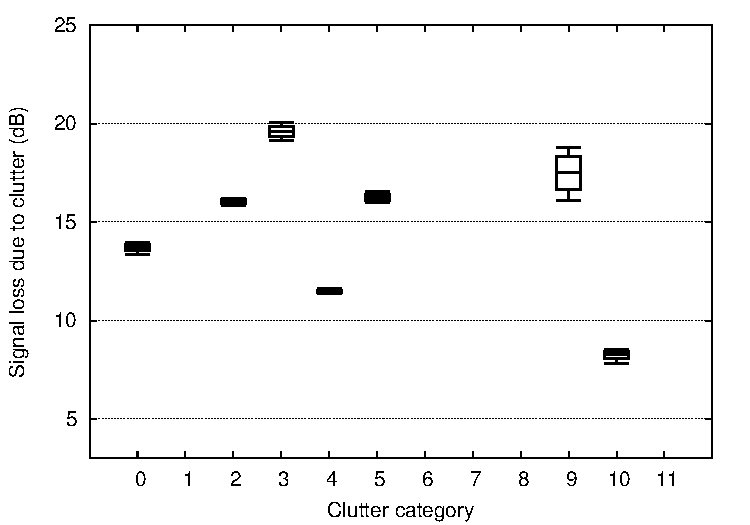
\includegraphics[width=0.65\textwidth]{\lyxdot \lyxdot /tun_par/doc/img/boxplot-MS}\\\hspace*{0.2in}(a)

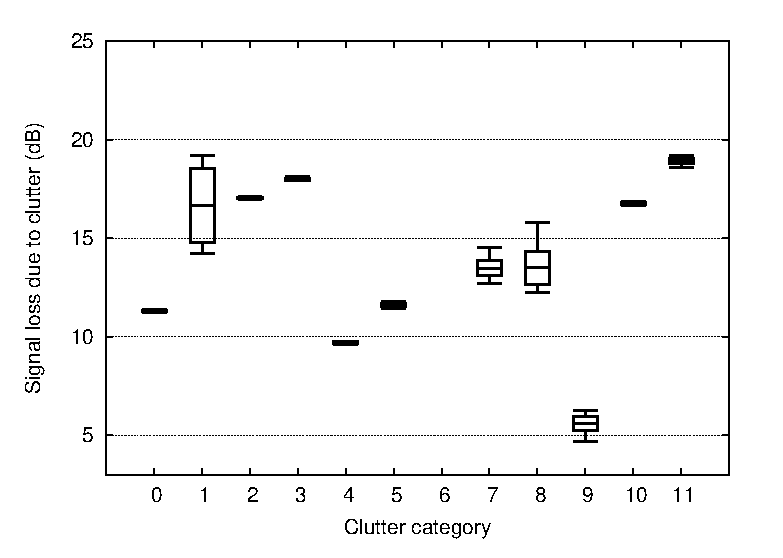
\includegraphics[width=0.65\textwidth]{\lyxdot \lyxdot /tun_par/doc/img/boxplot-LJ}\\\hspace*{0.2in}(b)

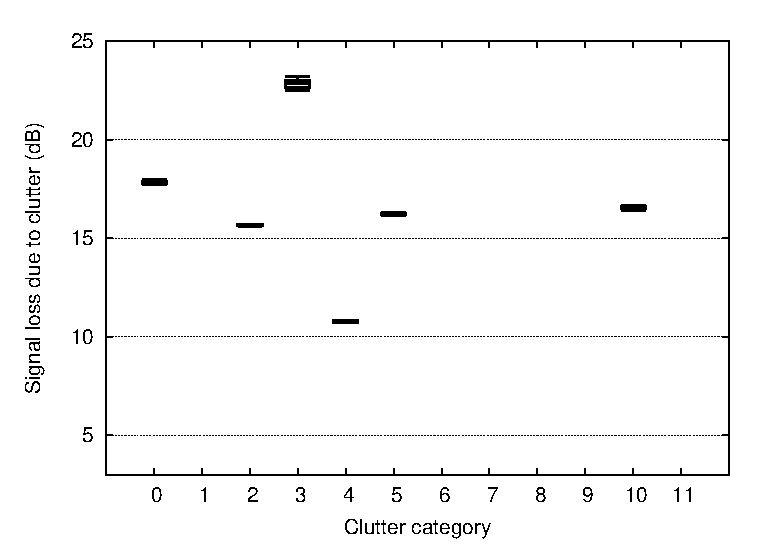
\includegraphics[width=0.65\textwidth]{\lyxdot \lyxdot /tun_par/doc/img/boxplot-HI}\\\hspace*{0.2in}(c)

\caption{Box plots representing the statistical-analysis values of Table~\ref{tab:05-Statistical_analysis_of_solutions},
for the solutions of the clutter-optimization process of each test
network: (a)~Net$_{8}$, (b)~Net$_{9}$, and (c)~Net$_{10}$.\label{fig:05-Statistical_analysis_boxplots}}
\end{figure}


\bigskip{}


Because of the stochastic nature of the DASA, the results of 30 independent
runs were collected in order to have enough data for them to be statistically
relevant. In other words, the robustness of the solutions that were
presented in the previous section is analyzed here.

To this end, Table~\ref{tab:05-Statistical_analysis_of_solutions}
shows the solutions reached by the DASA for each of three test networks.
The calculated signal losses are depicted with the minimum, maximum
and average values for every clutter category, along with their standard
deviations. Again, hyphens represent clutter categories for which
there were no field measurements available, and thus they could not
be optimized. In order to easily visualize the data shown in Table~\ref{tab:05-Statistical_analysis_of_solutions},
box plots based on the same values are provided in Figure~\ref{fig:05-Statistical_analysis_boxplots}.
It can be observed that the standard deviation is low for almost all
optimized categories, indicating a consistent convergence of the optimization
algorithm. However, some exceptions are noticeable, e.g., the category
9 in Net$_{8}$ and Net$_{9}$, representing water. In this case,
there was a significantly lower density of field measurements nearby
water trails, since none of the test networks lays by the sea. Regarding
the categories 1 (suburban area), 7 and 8 (dry open land area) of
Net$_{9}$, a lower proportion of field measurements over these areas
was identified, thus higher standard-deviation values appear.

Based on these findings, the standard deviation of the optimized clutter
losses can be considered an indicator of the field measurements required
by the optimization process, i.e., a higher standard deviation denotes
more field measurements are needed to optimize the target clutter
category.


\section{Summary}

This chapter illustrated the suitability of PRATO as a network-planning
tool by tackling two coverage-planning problems, which were tested
over the newly deployed LTE network in Slovenia. The first one involved
the parameter tuning of the empirical radio-propagation model using
a snapshot of field measurements. The second one considered the optimization
of the clutter losses over different regions of the country, therefore
automatically adapting them to the local conditions of the geographical
region of each network.

The combination of the aforementioned techniques with PRATO provides
an environment-adaptable framework for radio-network planning. This
delivers a tool with a considerable improvement of the solution accuracy
of the analyzed instances, especially if compared to traditional,
i.e., manual or semi-automated, coverage-planning methods.

Additionally, the simulation results indicate that PRATO is applicable
for planning and optimization of real-world radio networks, since
it is capable of simulating a large number of coverage configurations
in a feasible amount of time. In particular, several of the presented
instances show a large computational-time complexity, which is beyond
reach for a serial implementation of an automated approach. Moreover,
the parallelization capabilities provided by the framework create
new problem-solving possibilities, together with the automation of
tasks that have been traditionally done manually by the network engineers.
Furthermore, even computational-intensive tasks such as objective-function
evaluations for stochastic optimization are feasible if PRATO is used.

To the best of the author's knowledge, an automatic-optimization method
for the clutter losses of a geographical area has not yet been presented
in the related literature.
